%
% Apunte de Sistemas Operativos
% Copyright (C) 2014 Esteban De La Fuente Rubio (esteban[at]delaf.cl)
%
% Permission is granted to copy, distribute and/or modify this document
% under the terms of the GNU Free Documentation License, Version 1.3
% or any later version published by the Free Software Foundation;
% with no Invariant Sections, no Front-Cover Texts, and no Back-Cover Texts.
% A copy of the license is included in the section entitled "GNU
% Free Documentation License".
%
% Link: http://www.gnu.org/copyleft/fdl.html
%

% UNIX
\chapter{Unix}
\label{unix}
% http://www.bell-labs.com/history/unix/

``Unix (registrado oficialmente como UNIX\textsuperscript{\textregistered}) es un sistema operativo portable, multitarea y multiusuario; desarrollado, en principio, en 1969 por un grupo de empleados de los laboratorios Bell de AT\&T, entre los que figuran Ken Thompson, Dennis Ritchie y Douglas McIlroy.''\footnote{\url{http://es.wikipedia.org/wiki/Unix}}

MULTICS fue un sistema operativo previo a Unix en el cual también estaba vinculado AT\&T pero tuvo poco éxito debido a su pobre rendimiento. Debido a esto se comenzó a trabajar en un nuevo proyecto el cual tuvo como nombre original UNICS, pero fue cambiado posteriormente a Unix ya que su pronunciación en inglés era igual a la palabra \textit{eunuchs} (castrado), lo cual creo el juego de palabras que indicada que UNICS era un MULTICS castrado.

Desde el sistema operativo Unix se han basado diferentes sistemas operativos, tales como los descritos en el cuadro \ref{derivados_de_unix} y con más detalles en la figura \ref{fig:unix_history} \footnote{\url{http://en.wikipedia.org/wiki/File:Unix_history-simple.svg}} se puede apreciar a grandes rasgos los principales derivados.

\begin{table}[h]
	\centering
	\begin{tabular}{|c|c|c|c|}
		\hline
			Sistema Operativo		& Año		& Basado en 									& Tipo código \\
		\hline
			BSD									&	1978	& Unix												& Ambos \\
			System III					& 1980 	& Unix												& Cerrado \\
			System V						& 1982 	& System III									& Cerrado \\
			Sun OS							& 1982  & BSD													& Cerrado \\
			AIX									& 1985	& BSD y System V							& Cerrado \\
			HP/UX								& 1985	& System III									& Cerrado \\
			System V R4					& 1987	& Sun OS y BSD								& Cerrado \\
			Minix								& 1987	& Inspirado por Unix					& Abierto \\
			Linux								& 1990	& Inspirado por Unix y Minix	& Abierto \\
			Solaris							& 1991	& System V R4									& Cerrado \\
			FreeBSD							& 1992  & BSD													& Abierto \\
			NetBSD							& 1992 	& BSD 												& Abierto \\
			OpenBSD							& 1993 	& NetBSD											& Abierto \\
			MacOSX Server				& 1998	& NetBSD											& Cerrado \\
			MacOSX							& 2000	& MacOSX Server y FreeBSD			& Ambos \\
			OpenSolaris					& 2005 	& Solaris											& Abierto \\
		\hline
	\end{tabular}
	\caption{Derivados de Unix (años son aproximados)}
	\label{derivados_de_unix}
\end{table}

\begin{figure}[htbp]
\centering
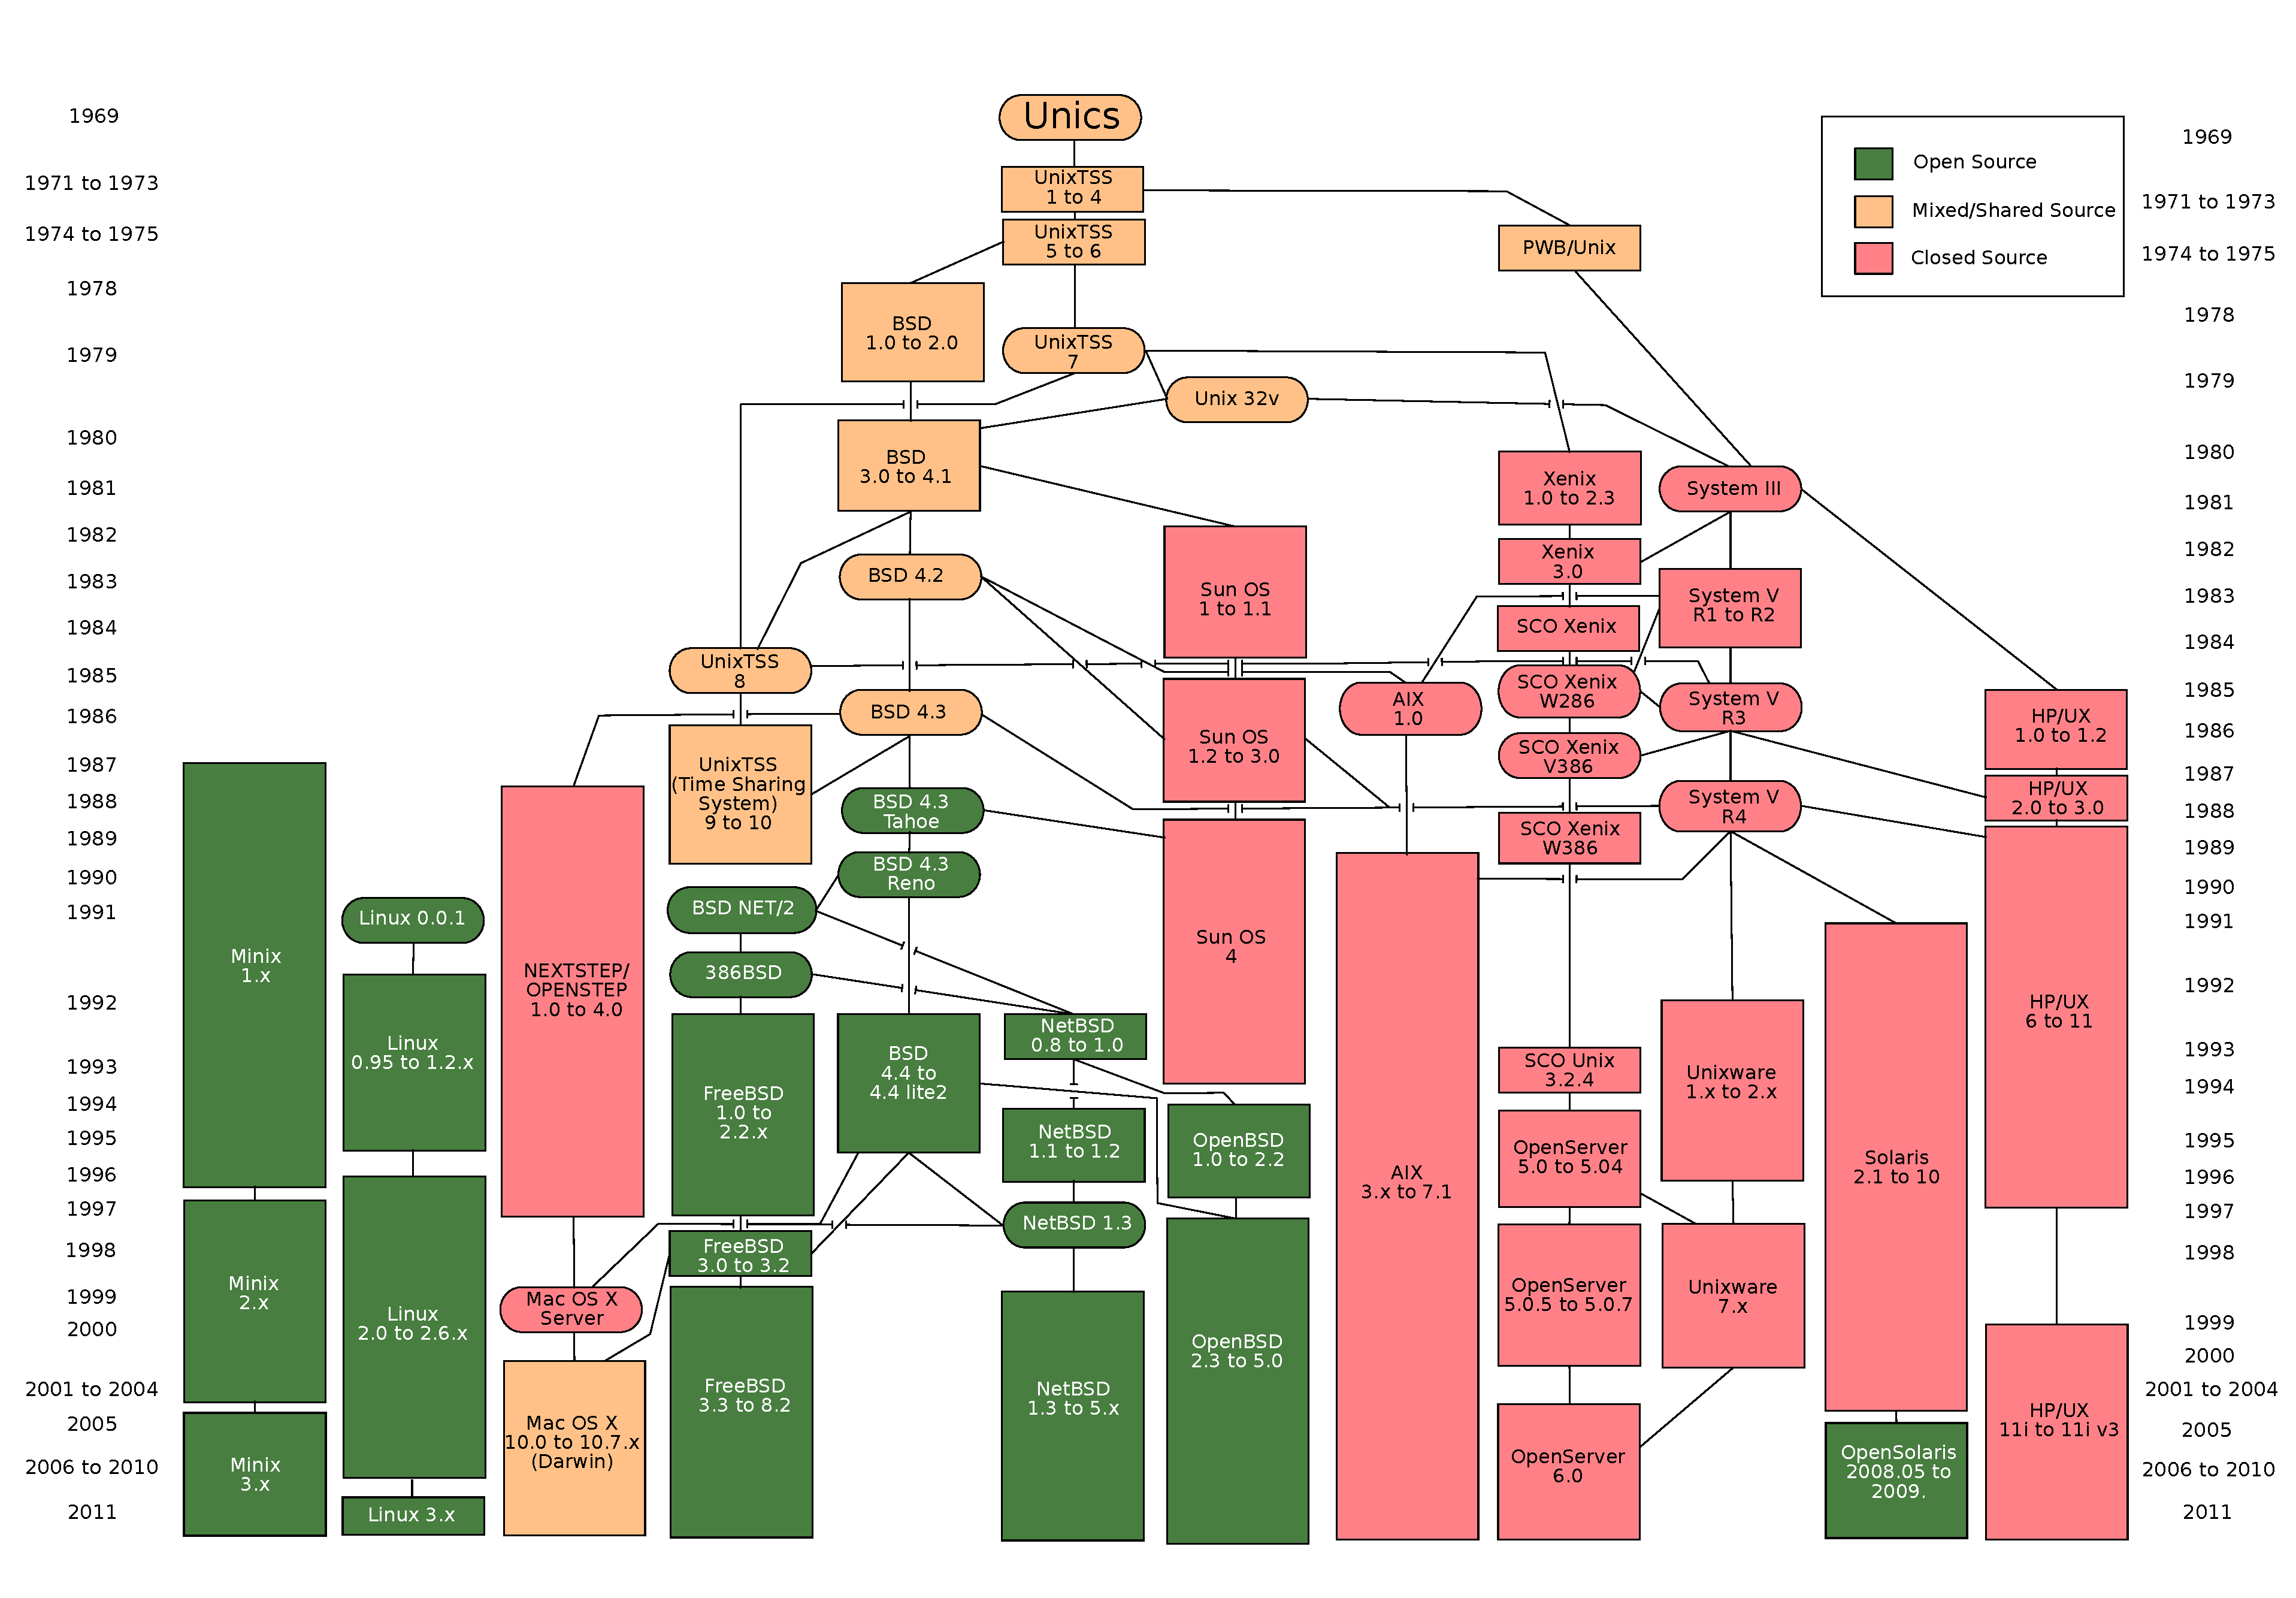
\includegraphics[scale=.30,angle=90]{img/unix/Unix_history-simple.pdf}
\caption{Mapa de la historia de Unix y sus derivados}
\label{fig:unix_history}
\end{figure}

Es importante destacar la participación de \textit{Berkeley Software Distribution} o BSD en la historia de los sistemas operativos \textit{like Unix}. La Universidad de California en Berkeley compró la licencia de Unix y empezó a hacer una variante del sistema operativo, implementando cosas que no venían por defecto con el primero. Un ejemplo de esto es el concepto de sockets, el cual no estaba presente en Unix y surgió en BSD. Posteriormente aparecieron diversas versiones de sistemas \textit{like Unix} basadas en BSD, muchas de ellas usados actualmente.

POSIX es un esfuerzo por estandarizar los distintos sistemas operativos \textit{like Unix}. De esta forma diferentes empresas podían escribir código común y que funcionase en las distintas plataformas. El problema en POSIX es que no consideraba todo lo que se podía realizar, un ejemplo de esto era que no se consideraban los hebras dentro del estándar y originalmente los sistemas POSIX corrían solo procesos pesados. Esto llevo a que no fuera un estándar completo y muchos desarrolladores programaran código fuera del estándar POSIX lo cual lo hacía menos portable.

\section{Tipos de núcleos}

Los distintos sistemas operativos se han divido básicamente en dos grupos: clásicos y modernos.

Los \textbf{núcleos clásicos}, como Unix V 3.x, BSD, Sun OS 4.x y Linux 1.x para implementar la exclusión mutua dentro del núcleo inhiben las interrupciones. Estos sistemas operativos están diseñados para funcionar sobre un único núcleo en la máquina (sistemas monoprocesador). Por lo anterior, siempre tendrán un hilo como máximo activo al mismo tiempo.

Al contrario, los \textbf{núcleos modernos} o núcleos multi hilos pueden ejecutar varios hilos al mismo tiempo (limitado por la cantidad de núcleos en la máquina). Ejemplos de estos núcleos son Unix V 4.x, Win/NT, Solaris 2 y Linux 2.x.

% TODO: de aquí al final
% esto es lo dificil del control 2 en la chile.
\section{Spinlock}

Primitiva de más bajo nivel donde se basan las otras primitivas de más alto nivel (como semáforos).

%Stack original de internet, lo que es TCP/IP fue escrito para BSD :-) uso de FreeBSD en redes!!
%El resto son ports para otros sistemas operativos ohhh

\section{Núcleo clásico}

Modo sistema:
\begin{itemize}
	\item Un solo hilo activo.
Cambios de contextos explícitos: un hilo llama al scheduler, no ocurre interrupción del timer dentro del núcleo para cambiar de hebra.
No hay data races.
No hay interrupciones: todo el código ejecutado está con las interrupciones inhibidas, por lo cual no se gatillan. Cuando se vuelva a la ejecución de la aplicación ahí se vuelven a habilitar.
\end{itemize}

Modo usuario:
Solo procesos pesados.
No se comparte memoria.
No hay acceso al segmento sistema (diagrama layout memoria).
La única forma de pasar a modo sistema es a través de una interrupción (usando, por ejemplo, instrucción en assembler int en procesadores Intel).
Entonces una llamada al sistema se implementa con una interrupción explícita.

% diagrama!!

Son llamadas al sistema read, fork y exit. malloc no es llamada al sistema, ya que todo lo que ocurre es en el área de datos, pero si lo es srbk\footnote{man sbrk} que cambia el tamaño del segmento de datos, haciendo posible que se pueda seguir pidiendo memoria.

\subsection{Segmento de sistema}

Segmento de sistema es caja negra para el proceso que se está ejecutando, independientemente de si es o no código abierto. El hacker quiere ejecutar su código en modo sistema :D

En el segmento de sistema se encuentra el vector de interrupciones

Existen buffers de entrada y salida, por ejemplo del disco, entonces read una de las ultimas tareas que haces es copiar de los buffers al segmento de memoria que se indico por el usuario como buffer en el segmento de usuario. Si read no verifica que el puntero de memoria pasado sea del área de datos del usuario un hacker podría pasar como puntero de memoria un área del segmento de sistema que es comunmente usada, así al usar read se podría copiar código malicioso en la zona que no se valido, y que luego será ejecutada cuando el sistema operativo pase por dicha zona. Siempre se deben validar que los parámetros pasados son parámetros válidos.

Están los descriptores del proceso.

Colas de procesos.

Pilas de procesos ligeros. % pero si estos son solo pesados, no existen multiples thread, estos solo existen dentro del núcleo para la administración de los procesos dentro del mismo. La memoria se comparte con otrosp procesos ligeros del núcleo que son peers a los procesos pesados correspondientes % ver diagrama mas abajo

En la zona de datos:
Variables globales.
Buffers para fread y fwrite
Heap para malloc/free.

Cuando se ejecuta codigo en segmento se utiliza una propia pila, las llamadas a sistemas son resueltas en el segmento de sistema utilizando una pila propia (confiable).

% diagrama núcleo clásico

Todas las máquinas que implementan el modo dual utilizan dos stack pointer, USP (user stack pointer) y SSP (system o supervisor stack pointer).

Suponiendo que el registro de stack pointer, un mismo registro, ejemplo el 15, se mapeara a USP o a SSP dependiendo del modo que se este ejecutando. De esta forma dependiendo del modo que se esté utilizando, se usará la pila del proceso o la pila de procesos ligeros en el 

Procesos ligeros en el núcleo, son non-preempive, porque al estar ejecutandose en modo sistema las interrupciones, en el núcleo clásico, están deshabilitadas.

\subsection{Relación con nSystem}

Unix													nSystem
Procesos pesados							Tareas de la aplicación (nTask)
Procesos ligeros							nTarea con señales inhibidas
Interrupción del TIMER				Señales SIGALARM (tiempo real), SIGVTALARM (tiempo cuando el proceso tiene la CPU)
Espacio direcciones virtuales	No está disponible
Interrupción inhibe otras interrupciones			START\_CRITICAL
Ejecución de reti							END\_CRITICAL

Una de las consecuencias es que dentro del núcleo todos los procesos son ligeros, o sea todos comparten memoria. A pesar de que Unix, desde el usuario, se ven procesos pesados, desde el punto de vista de la implementación, en la implementación de la llamada al sistema, el proceso se convierte en su contraparte (peer) proceso ligero. Dentro del núcleo los procesos se vuelven ligeros y son non-preemptive. % núcleo unix siempre ve tiempo real

Problema de este enfoque, las interrupciones pueden permanecer inhibidas por tiempo considerable (milisegundos) lo cual puede ser nefasto para ciertos dispositivos, sobre todo sistemas operativos en tiempo real, donde las interrupciones deben ser atendidas en un tiempo acotado. Esto se resolvía identificando cuales son las llamadas al sistema que pueden pasar mucho tiempo, y en esa se permitían otras interrupciones, esto complicaba ya que aparecían secciones críticas (como la cola de procesos listos). A pesar de lo anterior, dichas modificaciones eran aceptables.

En la versión 1 de linux, las puertas seriales tenian un buffer muy pequeño (de 1 byte) si no se atendían rápida, se podrían perder datos. Para evitar esto habían trucos que se usaban en el núcleo clásico se activaban las interrupciones solo para ejecutar aquellas de la puerta serial, solo esas se permitían junto a otras, esto para evitar perder datos.

Ventaja: simple, implementación con poco código (menos recursos, menos memoria)
Desventaja: no admite múltiples núcleos.

\section{Núcleos modernos}

¿Unix para multi núcleos?

Parchear: solo un núcleo puede estar trabajando en el núcleo. Pregunta, como se hace esperar? En la rutina de atencion de todas las interrupciones, se debe pedir un spinlock para evitar que exista mas de una ejecución del segmento de sistema en los nucleos. Esto permitirá que se ejecuten varios procesos, pero solo uno al mismo tiempo en modo sistema.

Otra forma es reescribir el codigo xD

%%%%% clase jueves 10/05

Unix para mono-procesadores
Mientras existe ejecución del código del núcleo en el procesador, este corre con interrupciones inhibidas. Como no hay otros \textit{cores} no habrán \textit{data races}.

\section{Unix en multi-procesador}

\begin{itemize}
	\item Inhibir las interrupciones no basta.
	\item Otros \textit{cores} sí pueden producir \textit{data races} en el núcleo.
	\item La visión del proceso del usuario no cambia: un solo procesador virtual, no se comparte memoria con otros procesos, entonces no hay \textit{data races}.
\end{itemize}

Soluciones:
\begin{itemize}
	\item Núcleo clásico: garantizar un solo \textit{core} ejecutando código del núcleo.
	\item Núcleo multi thread.
\end{itemize}

\subsection{Respecto al \textit{scheduling}}

En la práctica los cores tienen asignados procesos y estos tienen prioridad para acceder a cierto procesador. O sea, la cola de procesos ready es por core, más una cola global para cuando se acaban los procesos de dicha cola. Esto busca minimizar los cambios de un proceso de un core a otro, o sea la escritura de los datos en la cache de dicho core. Si P2 se está ejecutando en Core1, y luego Core2 quiere ejecutar P2, se deberán mover los datos desde el cache del Core1 al cache del Core2. Esto es bastante más complicado de implementar, por lo cual se considerará:

Hay un reloj regresivo (TIMER) por \textit{core}.
Se supondrá que la cola de procesos \textit{ready} es compartida.

¿Cómo encausar exclusión mutua en el núcleo? ¿Usar semáforos? (problema huevo y gallina). La solución a esto son los spin-locks.

\subsection{Spin-locks}

No son para sincronizar procesos, son para sincronizar a más bajo nivel, o sea, sincronización de cores. Solo tienen sentido al tener multicores.

Un spin-lock es un entero, que puede ser 0 o 1, indicando si esta libre o no el spin-lock.

\begin{verbatim}
#define OPEN 1
#define CLOSED 0
int lock;
\end{verbatim}

Un core deberá consulta por el estado del spin-lock, si esta tomado deberá esperar

\subsubsection{API}

\begin{verbatim}
void spinLock (int *plock) {
  while(*plock==CLOSED);
  *plock = CLOSED;
}

void spinUnlock (int *plock) {
  *plock = OPEN;
}
\end{verbatim}

La función spinLock presenta data races. Aquí no se pueden utilizar primitivas del sistema operativo, ya que esto es el sistema operativo. Se debe buscar algo de más bajo nivel.

Es difícil implementar exclusión mutua con solo lectura y escritura de memoria. Existen algoritmos pero son complejos, usando cosas como acceso secuencial de la memoria, sin embargo esto no está disponible en procesadores modernos por razones de eficiencia.

El hardware será quien entregará la sincronización a más bajo nivel. Procesadores ofrecen una instrucción para la lectura y escritura atómica de una palabra en memoria. De esta forma ningún otro procesador podrá hacer una operación mientras otro este trabajando sobre esa palabra en memoria.

En Sparc se llama swap:

swap dir, reg

Intercambia el contenido de la dirección (dir) con el del registro (reg)

En Intel existe test and set

% Ver código Linux donde están los spin-locks

Spark: Supongamos int swap (int *plock, int val) una función que retorna el valor antiguo de plock y lo cambia por val. Esta debe ser implementada en assembler usando la instrucción swap.

Solución correcta:
\begin{verbatim}
void spinLock (*plock) {
  while(swap(plock, CLOSED)==CLOSED);
}
\end{verbatim}

Como swap es atómico, si dos cores usan swap al mismo tiempo, uno de ellos verá el valor OPEN y el otro verá CLOSED.

Esta solución utiliza busy-waiting para revisar el valor del spin-lock. Para sincronizar cores no queda otra alternativa que hacer busy-waiting. Lo ideal sería ejecutar otro proceso, pero no se puede, porque para ejecutar otro proceso se tendría que acceder a la sección crítica (código del núcleo) que es por la cual estamos esperando.

Para la solución 1, un núcleo clásico tendrá un solo spin-lock para entrar a ejecutar el código del núcleo. El problema de esto es que es ineficiente, ya que swap hace acceso a la memoria de forma \textit{inútil} ocupando el BUS de datos.

Una mejora a lo anterior es usar la memoria caché, de tal forma que los cores van pidiendo la propiedad de la dirección de memoria de la RAM para poder transferirla a la cache. Supongamso que un C1 requiere el spin-lock (que esta OPEN), C1 pide la propiedad de la memoria, se le da, se copia a cache de C1 y se modifica, cuando llega un C2 pide la propiedad de la direccion y copia a cache, ahora cada lectura y escritura con swap en C2 se realizará en la memoria cache de C2. Esto funciona bien para 2 cores, sin embargo para más cores los cores ejecutarán swap para levar el spinlock a su cache y esto ocupara el BUS de datos.

Acceder a la cache requiere de 1 a 10 ns, en cambio para acceder al bus requeire 100ns. En este caso los cores C2 y C3 podrían usar todo el BUS y evitar que el core C1 con trabajo útil avance lento.

Solución más correcta
\begin{verbatim}
void spinLock (*plock) {
  while(swap(plock, CLOSED)==CLOSED)
    mini_loop(); /* instrucciones de cpu no útil (nop) */
}
\end{verbatim}

Los spin-locks son lo más eficiente cuando no hay contención (que un core quiera adquirir el spin-lock y estaba tomado). Idealmente hay que tomar  el spin-lock por tiempo breve (1 micro segundo).

Problema en un núcleo clásico: el tiempo en el núcleo puede no ser breve y podría ocurrir contención.
Idea: Se busca que en ciertos lugares del código del núcleo puedan haber varios cores ejecutando dicho código.
Solución en núcleo parcheado:
1) En lugares de uso intensivo de la CPU se admiten varios cores en el núcleo. Esto implica que si hay secciones criticas dentro de ese código se deberá volver a pedir el spin-lock.
2) Núcleo multi thread: se admite siempre varios cores en el núcleo.

Linux internamente usa semáforos para sincronizar aquellas situaciones de contención alta (más de un micro segundo por ejemplo), para casos de tiempo corto usa los Spin-locks.

La sugerencia académica es el uso de monitores para sincronizar dentro del núcleo.

El enter ... exit es de corto plazo, si se quiere hacer algo a largo plazo usar wait.

Implementación de monitores en un núcleo Unix multithreads.

\begin{verbatim}
typedef struct {
  int spinLock;
  kQueue *wq; /* wait queue */
} *kMon;

void kEnter (kMon m) {
  disable(); /* desactivar interrupciones */  
  spinLock(&m->spinlock);
}

void kExit (kMon m) {
  spinUnlock(&m->spinLock);
  enable(); /* activar interrupciones */
}

void kWait (kMon m) {
  kProcess p = kCurrentProcess();
  p->status = WAIT_MON;
  kPutProcess(m->wq, p);
  spinUnlock(&m->spinLock);
  kResume();
  spinLock(&m->spinLock); /* solicitar nuevamente la propiedad del monitor al ser despertado con notifyAll */
}

void kNotifyAll (kMon m) {
  spinLock(&ready_queue_lock); /* spinlock para acceder a la ready_queue */
  while() {
    kProcess = kGetProcess(m->wq);
    w->status = READY;
    kPut(ready_queue, w);
  }
  spinUnlock(&ready_queue_lock);
}
\end{verbatim}

% caso de cores duermiendo, espera, duerme, idle, etc
% como despertar a un core que esta duermiendo? interrupcion, el profe no sabe

% Ejercicio, como implementar un semáforo a partir de spin-locks. (pregunta de control)

La idea es que lo que se ejecute entre kEnter y kExit sea breve  y no tenga otros estados de espera, de tal forma que las interrupciones no estén deshabilitadas mucho tiempo.

\section{Entrada y salida (E/S)}
Unix leerá datos completos, lo primero que se hace en E/S es verificar si los datos están en los buffers, en caso que sea lea de un disco y no hayan más datos en el buffer (o sea lea de un socket) en dicho caso se programará al disco para que realice la lectura. Esto se hace mediante canales DMA, para leer y transferir a los buffers. Luego se hace un mapeo donde se indica que el proceso requiere leer datos del disco, se suspende el proceso en espera que se lean los datos. El disco luego generará una interrupción de hw cuando el disco termine de hacer la operación de lectura. donde se invocará una rutina de atención de interrupciones, el hw inhibe las otras interrupciones, y se revisa que disco genero la interrupcion y con que datos, esto para poder determinar quien estaba esperando los datos. Luego se pasa el proceso a modo ejecución con los datos en el buffer.

Todo esto se hace con el uso de los drivers del disco, los cuales manejan las partes dependientes del hw.

% En unix se pueden hacer intercepciones, donde si se llama a read, unix no ejecuta el read del sistema sino uno definido por el usuario EJEMPLO!
